
\chapter{Limpieza de datos: extracción de usuarios relevantes}
\label{chap:extraccion_de_usuarios}

Como hemos visto en el análisis exploratorio inicial de los datos, la fase 
de limpieza de la información va a ser muy relevante para conseguir
nuestro objetivo final. Se trata de extraer, a partir de los tuits almacenados, 
una lista de usuarios que pudieran constituirse en candidatos adecuados a 
una oferta de trabajo (como, por ejemplo, las de la figura \ref{fig:ofertas_descripcion}). 
Para ello, de todos aquellos usuarios de los que tenemos constancia en 
los tuits recogidos, hemos de seleccionar aquellos que sean personas (eliminando bots, 
empresas, etc.) y que hayan publicado contenido relacionado con la materia de referencia, 
en este caso la ciencia de datos.

Esquemáticamente, el proceso descrito en este capítulo es el siguiente:
\begin{enumerate}
\item Consideramos todos los tuits que hemos descargado, tanto los originales como los datos de los tuits que han sido retuiteados o citados en los originales.
\item Estudiamos los idiomas en que han sido escritos, y seleccionamos aquellos que usaremos en el 
análisis (sección \ref{sect:deteccion_idioma}).
\item Discriminamos los tuits cuyo contenido está relacionado con la ciencia de datos o el Big Data (los \lq\lq relevantes\rq\rq,  sección \ref{sect:tuits_relevantes}).
\item Consideramos los usuarios que han producido esos tuits de contenido relevante, quitando los repetidos
de forma consistente con el resto del proceso (ver detalles en la subsección \ref{subsect:duplicados1}). 
\item De los usuarios relevantes, seleccionamos aquellos que clasificamos como personas (sección 
\ref{sect:tipo_de_usuario}).
\item De aquellos usuarios clasificados como personas, de nuevo eliminamos los duplicados,
según el criterio expuesto en la sección \ref{subsect:duplicados2}.
\end{enumerate}

El resultado de este proceso será entonces una tabla de id de usuarios que procederemos más tarde
a ordenar en función de su relevancia.

Los desarrollos descritos en este capítulo están en el fichero {\bf Python/user\_selection.py}, 
que puede encontrarse en el repositorio de GitHub.


\section{Detección del idioma} 
\label{sect:deteccion_idioma}

El primer paso para poder analizar el contenido de un tuit y determinar si dicho tuit 
(y por tanto el usuario que lo ha publicado) está relacionado con la ciencia de datos o el big data,
es determinar el lenguaje en el que está escrito. Como ya hemos mencionado,
aunque la búsqueda en Twitter se realizó solicitando el campo \lq\lq languages = ["es"]\rq\rq,
obtenemos algunos tuits en otros idiomas, como estos dos 
que mostramos a continuación:

\myfigure{
\begin{tabular}{cc}

\includegraphics[width=0.4\textwidth]{tuit_ingles1}
&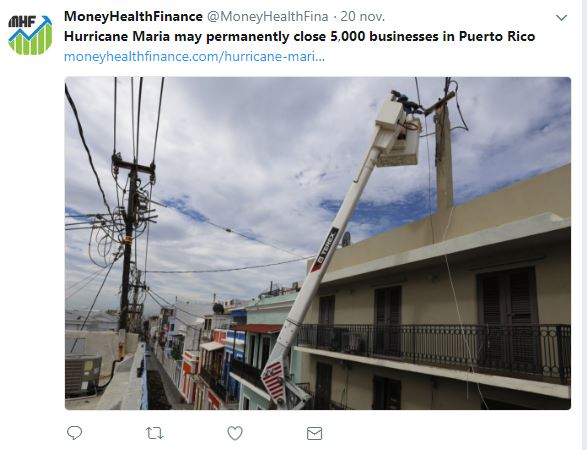
\includegraphics[width=0.4\textwidth]{tuit_ingles2}
\end{tabular}
\figcaption{Tuits no solo en español.}
\label{fig:tuits_ingles} }

Los primeros trabajos sobre el problema de la detección automática del lenguaje de un texto
se remontan a la década de 1970 \cite{zissman-berkling}. En la mayoría de las propuestas, 
existe una fase de entrenamiento, sobre textos previamente clasificados, en la que se produce 
un modelo del lenguaje (tal vez uno por lenguaje), y una fase de reconocimiento, en la que 
el lenguaje de mayor verosimilitud para el texto se extrae a partir de la aplicación de los 
distintos modelos. La clave de todos estos métodos es la modelización del lenguaje, algo que puede 
conseguirse atendiendo a diversas características diferenciadoras: fonemas, morfología, 
sintaxis y/o prosodia\footnote{Entonación, acento, melodía; relevante en el
caso de detección de idioma en textos hablados.}. 

La aplicación de dichas técnicas a textos provenientes de entornos web, blogs,  foros, etc. 
no está exenta de problemas, ver por ejemplo \cite{almeida_estevez_piad}.
Los textos procedentes de entornos web en general, y de Twitter en particular, 
presentan elevados niveles de lo que podríamos denominar como \lq\lq ruido\rq\rq,
por ejemplo:
\begin{itemize}
\item suelen ser textos cortos, lo que dificulta la aplicación de técnicas basadas en frecuencia 
de palabras o caracteres,
\item presencia de enlaces web, etiquetas, emoticonos y otros caracteres propios del entorno,
\item uso de jerga, lenguaje informal y palabras en idiomas distintos del principal del texto,
\item modificaciones de la ortografía, que van desde palabras abreviadas (\lq\lq q\rq\rq, 
\lq\lq xa\rq\rq) a expresiones enfáticas (\lq\lq mooooooolaaaaaaaa\rq\rq), por poner dos 
ejemplos.
\end{itemize}


A pesar de que es posible encontrar corpus de textos con estas características 
ya clasificados por 
idioma\footnote{\url{https://blog.twitter.com/engineering/en_us/a/2015/evaluating-language-identification-performance.html }}
que pudieran servir para entrenar un modelo que determinara el lenguaje,
hemos optado por usar un clasificador que no necesite entrenar un modelo, 
ya que esta parte del proyecto no es la principal. Hemos encontrado
referencias, como \cite{almeida_estevez_piad}, que apuntan al buen comportamiento de 
clasificadores que no dependen de conjuntos de entrenamiento (basados en \lq\lq small words\rq\rq,
también denominadas \lq\lq stop words\rq\rq, y trigramas). Este método requiere de una implementación
{\em ad-hoc}.

Hemos explorado las opciones disponibles, listas para usar, en el entorno de Python, 
y hemos encontrado varios paquetes que tratan el 
problema de detectar el idioma de un texto automáticamente. Los más
comentados son los siguientes:
\begin{itemize} 
\item {\tt langid} \cite{langid}: es un paquete que proporciona un 
clasificador Naïve Bayes de textos, que usa $n$-gramas (secuencias de $n$ caracteres en el texto, con $1\leq n\leq 4$). 
El clasificador está pre-entrenado sobre diversos corpus de texto, en un total de 97 idiomas. Según los
resultados explicados en el artículo de presentación del trabajo, es un método con una
exactitud ({\em accuracy}) del 94\%.
\item {\tt langdetect}: de Nakatani Shuyo, también es un clasificador Naïve Bayes basado en $n$-gramas, con
normalizaciones heurísticas, \url{https://github.com/shuyo/language-detection }.
\item {\tt LDIG}: es un clasificador específico para Twitter, creado por el autor
de {\em lagdetect} para solventar las carencias de éste en la clasificación de mensajes
cortos, \url{https://github.com/shuyo/ldig }. Soporta menos idiomas que los anteriores.
\item {\tt equilid}: es el paquete de más reciente creación que hemos encontrado,
que además está especialmente diseñado para tratar el \lq\lq ruido\rq\rq
que comentábamos caracteriza los textos de Twitter. Está concebido para identificar
dialectos urbanos y tratar correctamente expresiones de jerga.
\end{itemize}

Los resultados mostrados para estos modelos nos han parecido lo suficientemente
buenos para el objetivo que perseguimos en este apartado, y hemos decidido adoptar esta solución.
Dado el tema que nos ocupa, relacionado con ciencia de datos, la especialización 
de {\tt equilid} (no esperamos un lenguaje excesivamente alterado) 
y la dificultad de su instalación en el sistema disponible
(usa una versión de TensorFlow que aparentemente no está desarrollada para Windows),
nos hace descartarlo de entrada. 
En \cite{langid2} se muestra que el comportamiento de cualquiera de los clasificadores 
restantes es lo suficientemente bueno por
separado para el objetivo de este proyecto. Sugieren que combinar dos o más clasificadores
puede mejorar la exactitud de la clasificación, y que en general, la limpieza de
los tuits (urls, etiquetas, menciones, etc.), si bien mínimamente en algunos casos,
suele mejorar el comportamiento de los modelos (excepto en el caso de {\tt langid}). 
Finalmente, nos hemos decidido por usar el algoritmo del paquete {\tt langid}, visto
el buen resultado reportado, y la facilidad de uso del mismo. 

En \cite{langid2} se muestra que, en un contexto general de detección del lenguaje, 
el paquete {\tt langid} no parece beneficiarse de una limpieza del tuit
para retirar urls, menciones, etiquetas y emoticonos del cuerpo del mensaje.
Sin embargo, dado que la implementación de esa limpieza no 
es difícil, hemos comparado la clasificación del lenguaje obtenido
con el texto original y con el texto limpio, y hemos observado que en los
textos de los $24,128$ tuits descargados (contando retuiteados y citados también)
hay un $6.37$\% de tuits que no tienen la misma asignación de lenguaje. 
Estos tuits suelen ser tuits con pocas palabras
o con mucha mezcla de idiomas (generalmente español e inglés).

Como método alternativo, se ha implementado un clasificador manual que solo
usa \lq\lq stop words\rq\rq para tratar esos casos en los que {\tt langid}
no da una elección clara del idioma. Si el método de los \lq\lq stop words\rq\rq
da un idioma para el texto que coincide con alguno de los proporcionados por 
{\tt langid} (bien el del texto limpio, bien el del texto original), ese será
el que se asigne al tuit. Y si no, lo dejaremos clasificado con un idioma desconocido.

Hemos aplicado este método de clasificación del lenguaje a los $24,128$ textos
de los tuits originales, retuiteados o citados, y resulta una clasificación en $25$
idiomas diferentes. Mostramos a continuación un resumen de los resultados del clasificador:


\myfigure{
\begin{tabular}{cc}
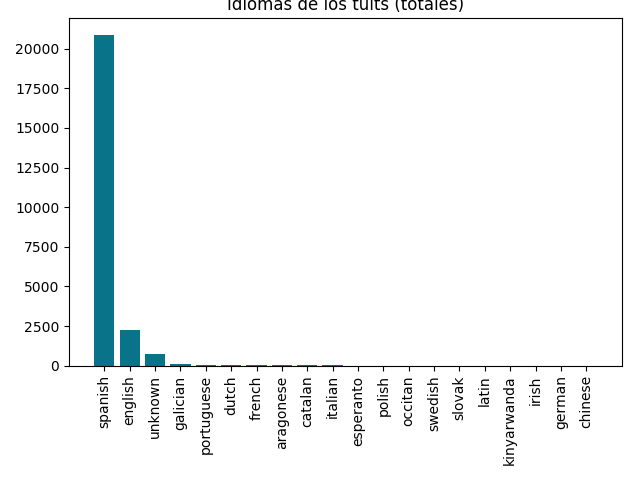
\includegraphics[width=0.4\textwidth]{C:/DATOS/MBIT/Proyecto/MBITProject_Data4all/Python/images/assigned_languages.png}
&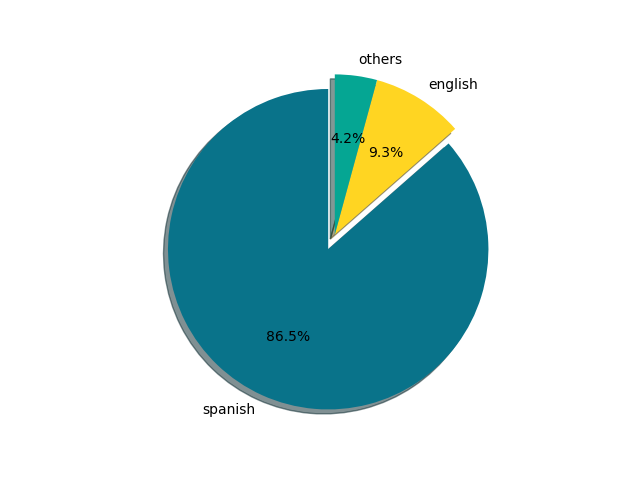
\includegraphics[width=0.4\textwidth]{C:/DATOS/MBIT/Proyecto/MBITProject_Data4all/Python/images/assigned_languages_proportions.png}
\end{tabular}
\figcaption{Clasificación por lenguaje del texto del tuit. Del $4.2$\% de \lq\lq others\rq\rq
hay un $2.9$\% de \lq\lq unknown\rq\rq.}
\label{fig:assigned_languages} }

Echando un vistazo a los resultados, aquellos que no están clasificados o que están
clasificados en idiomas poco probables, digamos, como el esperanto, son aquellos en los
que el clasificador seguramente ha fallado. Algunas veces parece ser porque casi no 
tuvieran texto o porque el texto contenga mucha mezcla de idiomas. Pero otras veces, 
como en el siguiente caso clasificado en esperanto, no está muy claro por qué:

\myfigure{
\begin{tabular}{cc}

\includegraphics[width=0.8\textwidth]{tuit_esperanto1}
\end{tabular}
\figcaption{Tuit clasificado como esperanto.}
\label{fig:tuit_esperanto1} }


{\bf Vistos los resultados del clasificador de lenguaje, usaremos para el análisis del 
contenido de los tuits los idiomas inglés y español.}

\section{Naturaleza del tuit}
\label{sect:tuits_relevantes}

En esta fase del proyecto el objetivo es discernir si el contenido del texto de un tuit que hemos
obtenido de Twitter a través de la búsqueda descrita en la sección \ref{sect:obtencion_datos},
es efectivamente relevante para seleccionar a su autor como un posible candidato
a la oferta de trabajo que nos ocupa.

El criterio para que un tuit tenga un contenido relevante será que describa o haga referencia
a alguna de las habilidades o conocimientos requeridos a los candidatos. Es decir, no 
basta con que el tuit hable de Big Data o de ciencia de datos en general, o de noticias 
relacionadas con ellos, sino tiene que mostrar algún signo de dichas habilidades y conocimientos.

Para ello, hemos desarrollado un modelo {\em ad-hoc} que pasamos a describir a continuación.

\subsection{Construcción del modelo}
\label{sect:construccion_modelo_tuits_relevantes}
En este apartado hemos elegido la opción de un {\bf modelo supervisado} con el objetivo de tener más eficiencia en la selección de usuarios relevantes.
Por otro lado, la clasificación de los
tuits mediante un modelo no supervisado (tipo \lq\lq bag of words\rq\rq, por ejemplo), 
es una técnica que ya exploramos en la clasificación del idioma del tuit que hemos 
tratado en la sección anterior, y en la clasificación del perfil de usuario que trataremos
a continuación.  

En la figura \ref{fig:tuit_content_model_flow} se describen esqumáticamente los pasos que hemos llevado a cabo para construir el modelo:

\myfigure{
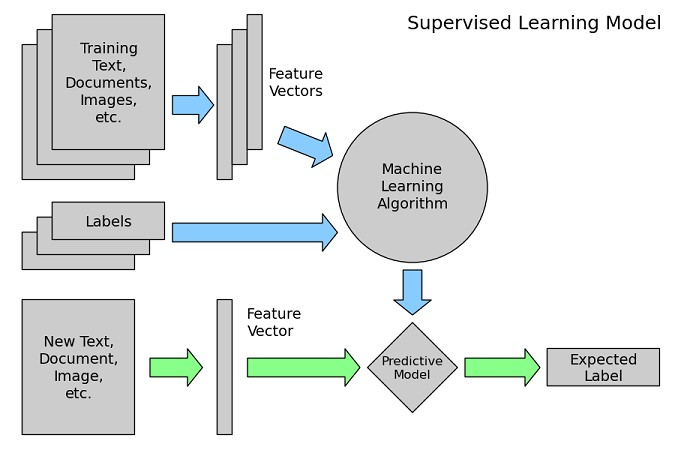
\includegraphics[width=0.8\textwidth]{tuit_content_model_flow}
\figcaption{Proceso de construcción y funcionamiento del modelo para clasificación de textos.}
\label{fig:tuit_content_model_flow} }



\subsubsection{Textos de entrenamiento}

Obtuvimos una nueva base de datos de Twitter con $50000$ tuits, con una búsqueda distinta
a la descrita en la sección \ref{sect:obtencion_datos} pero también por palabras clave,
a través del API Search de Twitter, y procedimos como en el caso
de la base de datos para la extracción de candidatos, a almacenarla en local en una base de MongoDB.


\subsubsection{Etiquetado del texto}
Trabajamos sobre esa base de datos para construir un data frame que contuviera los textos de los tuits,
así como otra información relevante de los tuits (aunque luego no se usa en el modelo), y procedimos
a etiquetar manualmente $2000$ de esos tuits. Los tuits etiquetados están almacenados en un fichero
Excel {\bf Python/relevance\_model/ds\_sample2.xlsx} de nuestro repositorio de GitHub.
Como curiosidad, nos gustaría comentar que al bajar los tuits por palabras claves como Python o SAS, 
obtuvimos tuits que hablaban de serpientes o de los problemas del Sistema Andaluz de Salud. 

\subsubsection{Limpieza de los tuits}
Antes de entrenar el modelo, intentamos eliminar el \lq\lq ruido\rq\rq de los textos 
sobre los que se va a realizar, sometiéndolos a una limpieza en la que retiramos
de los mismos urls, números, signos de puntuación, \lq\lq stop words\rq\rq, palabras de menos
de dos letras y distinción entre mayúsculas y minúsculas.
La función que lleva a cabo esta limpieza está hecha {\em ad-hoc}, y puede encontrarse en el
archivo {\bf Python/relevance\_model/Clasification1.py} de nuestro repositorio de GitHub:

\myfigure{
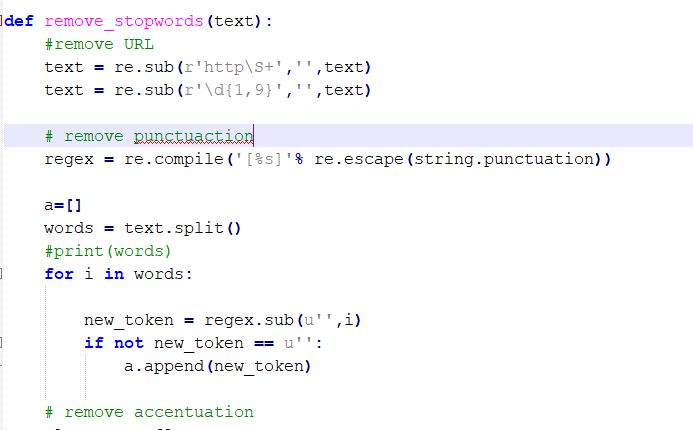
\includegraphics[width=0.7\textwidth]{clean_text_relevance_model}
\figcaption{Función para limpiar los tuits y entrenar el modelo de clasificación.}
\label{fig:clean_text_relevance_model} 
}
\subsubsection{Vector de características}
Los métodos y algoritmos usados 
en el entrenamiento y predicción con este modelo son
los que nos ofrece el paquete {\tt  scikit-learn} de Python. 

Los estimadores implementados en {\tt  scikit-learn}
necesitan transformar las palabras en vectores de características. Para eso elegimos el método {\tt TfidfVectorizer},  porque los textos de tuits son imprevisibles y el algoritmo TF-IDF ajusta la situación de que hay palabras que son más comunes y menos relevantes, además de ser  altamente recomendado en análisis de textos por su facilidad de uso y su parametrización. 
  
Este método convierte una colección de textos
a una matriz de características TF-IDF. Para ello, crea un  \lq\lq vocabulario\rq\rq 
con las palabras que aparecen en los textos y sus características TF-IDF en forma de diccionario.
En nuestro contexto, los niveles o características TF-IDF, son números que reflejan la 
importancia de cada palabra, de forma proporcional a la frecuencia en la que
aparece en el documento, pero  penalizados por la frecuencia total de ocurrencia 
de la palabra en todo el corpus. Más concretamente, \cite{notas_alvaro}, 
para cada palabra $t$ y cada documento $d$:

$$\begin{array}{rcl}
tf(t,d) &=& \left\{\begin{array}{ll}
1+\log_2(frec(t,d)) &\mbox{ si }frec(t,d)>0\\
0&\mbox{ en otro caso.}
\end{array}\right.\\
idf(t) &=& \log\frac{|D|}{|D_t|},
\end{array}
$$
donde
\begin{eqnarray*}
frec(t,d) &&\mbox{ es el número de veces que aparece $t$ en $d$}\\
D&& \mbox{ es la colección de todos los documentos }\\
D_t&& \mbox{ es la colección de los documentos que contienen la palabra }t\\
|A| && \mbox{ es el cardinal del conjunto }A.
\end{eqnarray*}
Finalmente, el TF-IDF de un par palabra-documento es
$$tfidf(t,d)=tf(t,d)*idf(t).$$

El resultado del método {\tt TfidfVectorizer}aplicado a un corpus, 
es una matriz en la que cada documento
del corpus es codificado como un vector cuyas entradas son los índices TF-IDF de cada
una de las palabras de dicho documento, con respecto a ese mismo documento.

Con esta manera de codificar los textos de los tuits, ya podemos entrenar un modelo 
de clasificación.

\subsubsection{Algoritmo de machine learning}
Para entrenar el modelo, dividimos esta muestra codificada en un $30$\% de datos de test y los restantes datos de entrenamiento,
y con esta división procedimos a entrenar el modelo.

Nos hemos decidido por un modelo de tipo Naïve Bayes, que 
invocaremos a través del modelo {\tt MultinomialNB()} de {\tt  scikit-learn}. Después de buscar e investigar, concluimos que este algoritmo,  aunque sea uno de los algoritmos más sencillos (lo que también hace que sea más fácil de usar y comprender), tiene muy buen desempeño, velocidad de procesamiento y funciona muy bien en clasificación de textos, por ejemplo al clasificar spam (\cite{notas_antonio}, \cite{nltk_book}).

Un modelo de clasificación de tipo Naïve Bayes, \cite{notas_antonio}, se basa en asignar
a cada observación aquella clase o resultado de la clasificación, a la que es más probable que
pertenezca, dados los datos que componen la observación. En concreto, nuestras observaciones
están definidas por una serie de variables $X_1, X_2, X_3,\dots$, y queremos adivinar para cada
observación el valor de otra variable $Y$ (discreta y finita).
En un modelo Naïve Bayes, el valor de $Y=y_i$ 
que asignaremos a una observación $(x_1, x_2,x_3,\dots)$ es aquel que hace máxima
$$P(Y=y_i|X_1=x_1,X_2=x_2,X_3=x_3,\dots).$$
Por la fórmula de Bayes,
\begin{eqnarray*}
\lefteqn{P(Y=y_i|X_1=x_1,X_2=x_2,X_3=x_3,\dots)}\\
 &=& \frac{P(X_1=x_1,X_2=x_2,X_3=x_3,\dots|Y=y_i)P(Y=y_i)}
{P(X_1=x_1,X_2=x_2,X_3=x_3,\dots)}\\
&=&\frac{P(X_1=x_1,X_2=x_2,X_3=x_3,\dots|Y=y_i)P(Y=y_i)}
{\sum_jP(X_1=x_1,X_2=x_2,X_3=x_3,\dots|Y=y_j)P(Y=y_j)}
\end{eqnarray*}
El cálculo de todas estas probabilidades condicionadas en la muestra puede ser muy costoso. El nombre 
de Naïve en el método viene de la simplificación que el método Naïve Bayes adopta para
llevar a cabo estos cálculos, y que consiste en suponer que 
las variables  $X_1=x_1,X_2=x_2,X_3=x_3,\dots$
son independientes entre sí. En ese caso, 
$$P(X_1=x_1,X_2=x_2,X_3=x_3,\dots|Y=y_i) = \prod_i P(X_i=x_i|Y=y_i),$$
y el cálculo se aligera notablemente. Sin embargo, esta hipótesis es generalmente la que más
problemas nos puede dar con estos modelos, \cite{nltk_book}, debido a que es muy poco habitual
en los problemas reales que las características sobre las que construimos el modelo sean 
independientes.

Según la documentación de {\tt  scikit-learn} sobre el modelo {\tt MultinomialNB()}\footnote{\url{http://scikit-learn.org/stable/modules/generated/sklearn.naive_bayes.MultinomialNB.html }},
este modelo en principio debería usarse para la clasificación con características discretas
(por ejemplo, conteo de palabras en el caso de clasificación de textos), ya que la distribución
multinomial normalmente requiere valores discretos. Sin embargo, en la práctica, 
conteos no enteros, como el del TF-IDF, también funcionan.


Las siguientes líneas de código son las que hacen el trabajo de entrenamiento del modelo:

\myfigure{
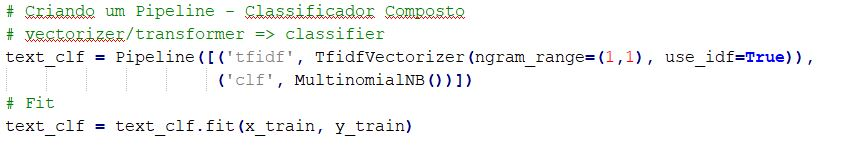
\includegraphics[width=0.7\textwidth]{model_training}
\figcaption{Código para el entrenamiento del modelo de clasificación de relevancia.}
\label{fig:model_training} 
}


\subsubsection{Uso del modelo}
Una vez entrenado el modelo, lo queremos usar en dos fases: en esta de selección de 
usuarios y en una posterior para la ordenación de los candidatos (ver sección 
\ref{subsect:indice_h}). Por ello, hemos guardado el modelo para 
exportarlo al fichero {\bf Python/relevance\_model/modelo\_clf.sav}
y tener la ocasión posteriormente de importarlo de nuevo. El uso que
vamos a hacer del modelo para clasificación es entonces a través de 
una importación:

\myfigure{
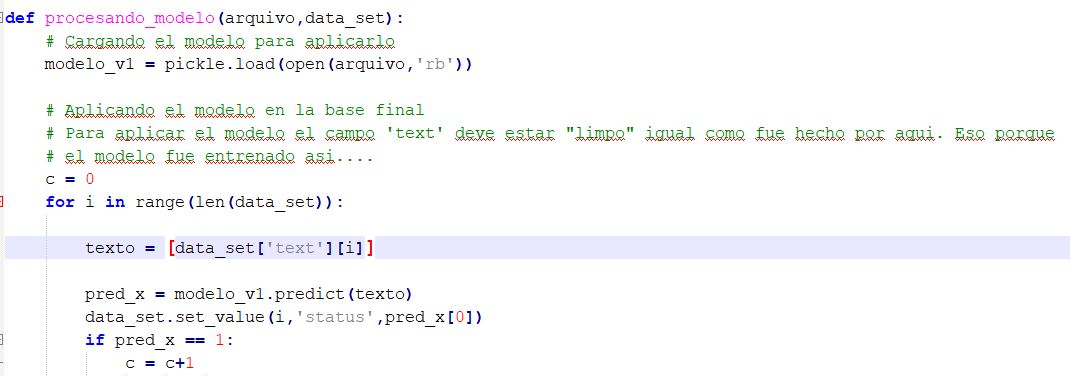
\includegraphics[width=0.7\textwidth]{model_use}
\figcaption{Código para usar el modelo Naïve Bayes de clasificación de contenidos ya 
entrenado en {\bf Python/relevance\_model/Clasificacion1.py}.}
\label{fig:model_use} 
}

Previo a predecir con el modelo, los textos han de pasar por el mismo proceso de 
limpieza que aquellos textos con los que se entrenó el modelo. Antes de llamar
a esta función, hay que procesar los textos sobre los que vamos a aplicarlo:

\myfigure{
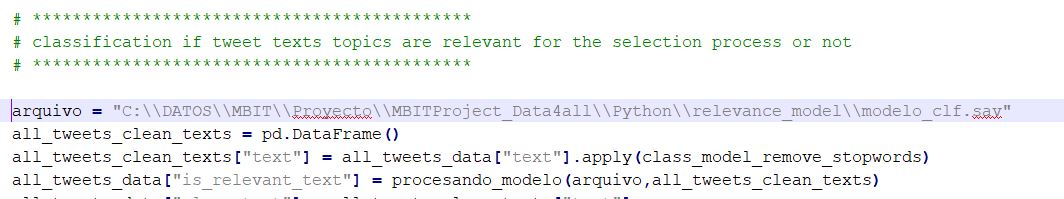
\includegraphics[width=0.7\textwidth]{cleaning_before_classification}
\figcaption{Código para limpiar los textos y posteriormente usar el modelo Naïve Bayes de clasificación de contenidos ya entrenado en {\bf Python/user\_selection.py}.}
\label{fig:cleaning_before_classification} 
}

\subsection{Evaluación del modelo de clasificación}
\label{sect:ajuste_modelo_contenido_tuit}

\begin{wrapfigure}[14]{L}{0.5\textwidth}
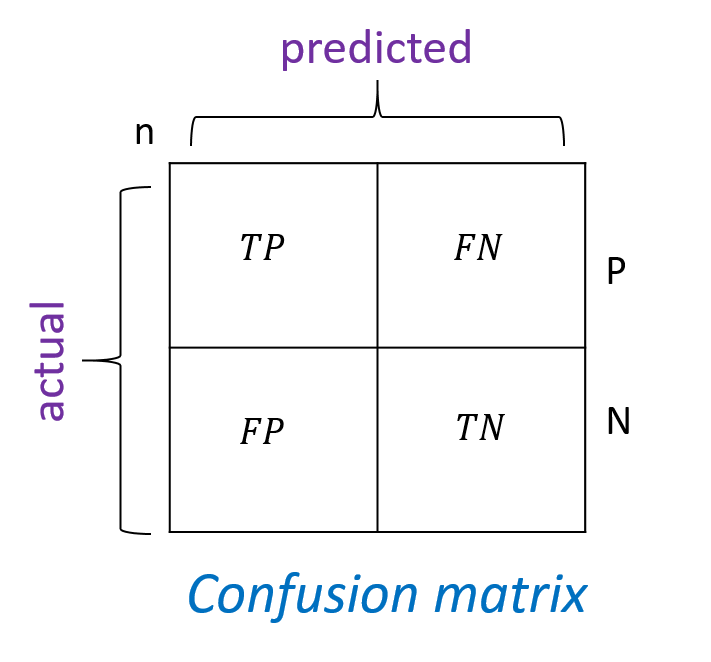
\includegraphics[width=0.45\textwidth]{confussion_matrix_definition}
\caption{Definición de la matriz de confusión.}\label{fig:confussion_matrix_definition}
\end{wrapfigure} 

Para entender mejor como está funcionando el modelo  tenemos las métricas de precision, recall, f1-score y la matriz de confusión. Recordemos la terminología que vamos a usar:
\begin{itemize}
\item[$TP$]: \lq\lq true positive\rq\rq: observaciones clasificadas correctamente en la clase positiva.
\item[$TN$] \lq\lq true negative\rq\rq: observaciones clasificadas correctamente en la clase negativa.
\item[$FP$] \lq\lq false positive\rq\rq: observaciones clasificadas incorrectamente en la clase positiva.
\item[$FN$] \lq\lq false negative\rq\rq: observaciones clasificadas incorrectamente en la clase negativa.	 
\end{itemize}
Con esta matriz de confusión obtenemos las siguientes métricas:
\begin{itemize}
\item Precisión: mide cómo de preciso es el modelo para detectar verdaderos positivos, y se define como
$$Pr = \frac{TP}{TP + FP}$$ 

\item Recall (sensibilidad): tasa de verdaderos positivos, mide la sensibilidad del modelo para detectar los positivos 	
$$Rc = \frac{TP}{TP + FN}$$ 
\item F1-Score: es una métrica más completa para medir la eficiencia del modelo, y se define como:
$$F1 = \frac{2Pr Rc}{Pr+Rc}.$$ 
\end{itemize}

En nuestro caso, los resultados del modelo entrenado sobre los datos de test son los siguientes:

\begin{center}
\begin{tabular}{ccc}

\begin{tabular}{r|cc}
\multicolumn{3}{c}{\bf Matriz} \\
\multicolumn{3}{c}{\bf de confusión} \\
\hline
\hline
     &$1$&$0$\\
\hline
$1$&$11$&$61$\\
\hline
$0$&$12$&$516$\\
\hline
\end{tabular}

&$$\hspace{2cm}

&\begin{tabular}{r|cccc}
\multicolumn{5}{c}{\bf Métricas de clasificación} \\
\hline
\hline
&Precisión &Recall&F1-score&Support\\
\hline
$0$&$0.89$&$0.98$&$0.93$&$528$\\
\hline
$1$&$0.48$&$0.15$&$0.23$&$72$\\
\hline\hline
Avg/total&$0.84$&$0.88$&$0.85$&$600$\\
\hline
\end{tabular}

\end{tabular}
\end{center}

Hemos calculado también la curva ROC, obteniendo
una exactitud (\lq\lq accuracy\rq\rq)
de $0.842500526094$, y la siguiente curva ROC:

\myfigure{
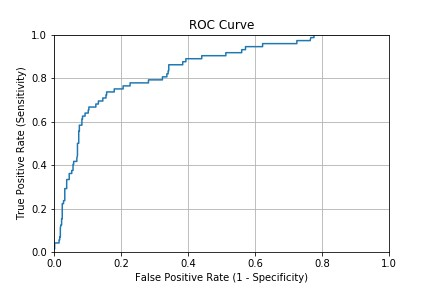
\includegraphics[width=0.7\textwidth]{first_ROC_curve}
\figcaption{Curva ROC del modelo de clasificación de textos según su relevancia.}
\label{fig:first_ROC_curve} 
}

Aceptamos estos primeros resultados y decidimos empezar el proyecto con este modelo para hacer las pruebas hasta el final. Sin embargo, estamos seguros de que es posible mejorarlo, principalmente en la precisión de los aciertos en la clase positivas ($TP$) y en la curva ROC, para lo cual hemos empezado a hacer pruebas con otros algoritmos y métodos de optimización (ver sección \ref{sect:mejoras_alg_clasificacion_tuit}).


\subsection{Resultados de la clasificación del contenido del tuit}
De los $24128$ tuits analizados, hemos encontrado $365$ cuyo contenido hemos clasificado como
re\-le\-van\-te, lo que representa un $1.51$\% del total. 
Los siguientes tuits fueron clasificados como no relevantes:

\myfigure{
\begin{tabular}{cc}

\includegraphics[width=0.4\textwidth]{text_not_relevant1}
&
\includegraphics[width=0.4\textwidth]{text_not_relevant2}\\

\includegraphics[width=0.4\textwidth]{text_not_relevant3}
&
\includegraphics[width=0.4\textwidth]{text_not_relevant4}\\
\end{tabular}
\figcaption{Tuits no relevantes.}
\label{fig:tuits_no_relevantes} 
}

Y los siguientes tuits fueron clasificados como relevantes:

\myfigure{
\begin{tabular}{cc}

\includegraphics[width=0.4\textwidth]{relevant_text1}
&
\includegraphics[width=0.4\textwidth]{relevant_text2}\\
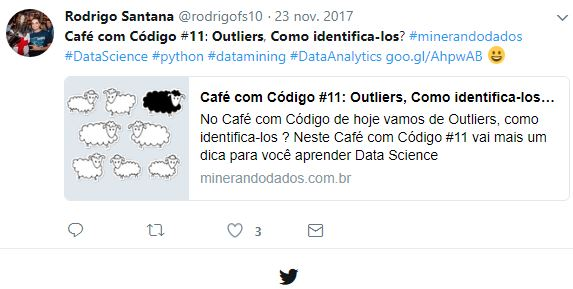
\includegraphics[width=0.4\textwidth]{relevant_text3}
&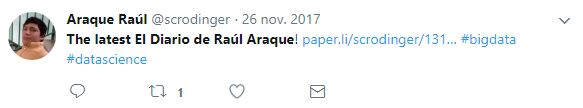
\includegraphics[width=0.4\textwidth]{relevant_text4}\\
\end{tabular}
\figcaption{Tuits relevantes.}
\label{fig:tuits_relevantes} 
}

\subsection{Listado de usuarios únicos}
\label{subsect:duplicados1}

El resultado del proceso que acabamos de describir
es una lista de tuits clasificados como relevantes o no relevantes
para nuestro propósito (encontrar candidatos para un puesto de científico de datos).
Nos quedaremos naturalmente solo con aquellos que hayamos clasificado como relevantes.

En esta lista de tuits relevantes, es razonable esperar que haya algunos 
publicados por el mismo usuario. Para optimizar la ejecución
del siguiente tramo del proceso, la selección de aquellos usuarios que son personas, 
de la lista de usuarios que podemos extraer de aquellos tuits que hemos clasificado como
relevantes, nos vamos a quedar solo con instancias únicas de los usuarios.

A lo largo de los procesos descritos en este capítulo y en el capítulo
\ref{chap:ordenacion_de_usuarios},
la referencia que vamos a usar para seguir a los usuarios es el número de identificación 
de usuario de Twitter, al que nos referiremos habitualmente como id.
Sin embargo, no es conveniente en esta etapa del proceso, quitar simplemente los id 
repetidos. Como veremos en la sección \ref{sect:tipo_de_usuario}, algunos campos relevantes
para la clasificación de un usuario en persona o no persona, son 
la url, el nombre de usuario y la descripción del usuario. Todos estos campos
pueden ser modificados por el usuario, y podría darse el caso de haber descargado
tuits de un mismo usuario, en el que aparecieran diferentes url, nombre de usuario o
descripción.

Dado que un usuario podría clasificarse de forma distinta con diferentes url, nombre de usuario y 
descripción, en esta etapa vamos a considerar que un usuario es un usuario repetido si para dos 
usuarios sus url, nombres de usuario, descripciones y por supuesto sus id, son iguales.

En el proceso de selección de usuarios, el origen del tuit (el canal o herramienta a través del que 
se publicó) también va a ser una característica relevante del proceso, pero solo para detectar bots. 
Al quedarnos con los usuarios únicos, hemos elegido no tomar en consideración el valor de
este campo, ya que en principio, un bot siempre publicará desde una fuente automática.


\subsection{Listado final de usuarios}
De los $365$ tuits cuyo contenido es relevante, podemos extraer $231$ usuarios cuyos campos
\lq\lq user\_id\rq\rq, \lq\lq url\rq\rq, \lq\lq user\_name\rq\rq y \lq\lq user\_bio\rq\rq
no están duplicados. Estos $231$ usuarios son los que pasarán la fase de análisis descrita a continuación.


\section{Tipo de usuario}
\label{sect:tipo_de_usuario}

Para clasificar al usuario respecto a su entidad, y por ejemplo distinguir entre personas, bots y empresas, 
una de las partes del tuit que más información contiene, a partir de los datos conseguidos, es
la descripción que los propios usuarios aportan. Antes de cualquier labor de análisis de esos textos,
es necesario saber el idioma en el que están, y por ello de nuevo aplicamos a nuestros datos 
el identificador de lenguaje que usamos en el apartado anterior. 

Primero seleccionamos los datos correspondientes a los usuarios distintos, obteniendo
$7,210$ usuarios con distinto \lq\lq{\em id\_str}\rq\rq. {\tt langid} clasifica de 
forma diferente el idioma de los datos de perfil antes y después de 
limpiarlos (quitar urls, emojis, hashtags, etc.) en un $5.99$\%
de los casos. Después de aplicar en éstos últimos el método de las \lq\lq stop words\rq\rq, 
los perfiles de los usuarios han quedado clasificados en $44$ idiomas diferentes.

\myfigure{
\begin{tabular}{cc}
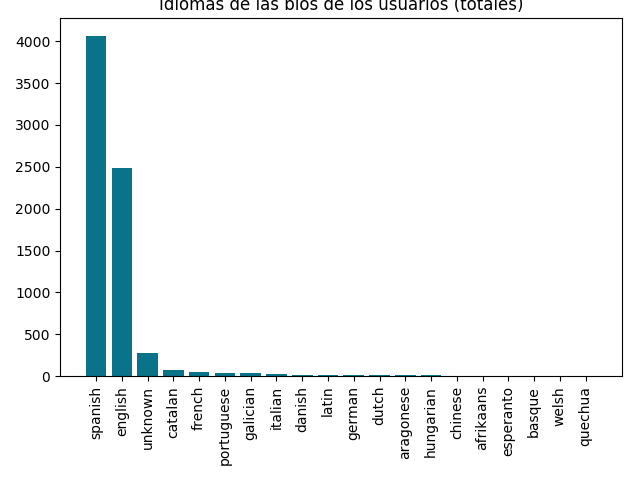
\includegraphics[width=0.4\textwidth]{C:/DATOS/MBIT/Proyecto/MBITProject_Data4all/Python/images/user_bios_assigned_languages.png}
&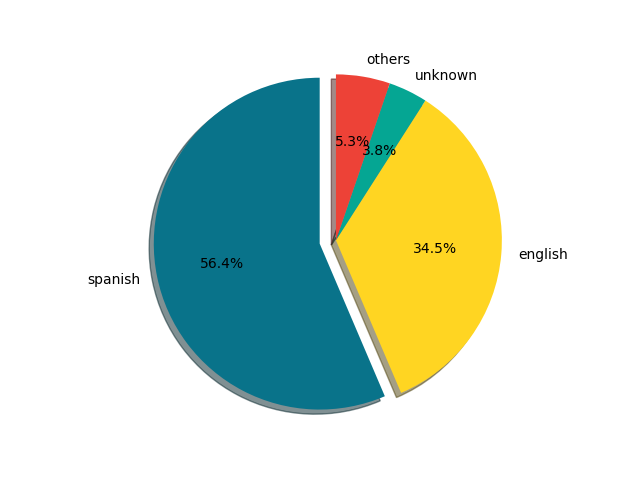
\includegraphics[width=0.4\textwidth]{C:/DATOS/MBIT/Proyecto/MBITProject_Data4all/Python/images/user_bios_assigned_languages_proportions.png}
\end{tabular}
\figcaption{Clasificación por lenguaje del texto de las bios.}
\label{fig:user_bios_assigned_languages} }

{\bf De nuevo, vistos los resultados del clasificador de lenguaje, usaremos para el análisis del tipo 
de usuario los idiomas inglés y español.}

\subsection{Revisión de la literatura}

Para poder hacer una ordenación de los candidatos necesitamos seleccionar a los usuarios o personas 
reales y tratar dos temas. Por un lado separar a personas y empresas y por otro eliminar los bots 
o perfiles automatizados.

Bajo el nombre de \lq\lq empresas\rq\rq, nos referimos a organizaciones o entidades asociadas con algún objetivo social, político o comercial que, a menudo, tienen una cuenta de Twitter por diversas razones, como
la gestión de las relaciones públicas o el servicio al cliente, entre otras.
Las organizaciones pueden ser de carácter comercial (por ejemplo, una empresa de marketing) o 
sin ánimo de lucro (por ejemplo, una ONG) y podrían incluir una empresa, marca, producto o institución benéfica 
(\cite{user_class7}). 

Las personas comunes son usuarios que probablemente estén en Twitter por diversos motivos, 
como publicar actualizaciones sobre su vida cotidiana, ampliar oportunidades profesionales, 
mantener contactos con sus amigos y conocidos o descubrir contenido relevante relacionado con sus intereses
(\cite{user_class7}).

En Internet, un \lq\lq bot\rq\rq  (aféresis de robot), \lq\lq web robot\rq\rq, \lq\lq WWW robot\rq\rq o 
\lq\lq Internet bot\rq\rq, es una aplicación que realiza de forma autómatica diversas 
tareas en la red\footnote{\url{https://en.wikipedia.org/wiki/Internet_bot}}.
En las redes sociales en general, los bots se utilizan para simular la interacción humana, 
hinchando artificialmente el número de visitas o seguidores, o automatizando respuestas 
para posicionar mensajes o influir en debates.
En Twitter\footnote{\url{https://en.wikipedia.org/wiki/Twitter_bot}} en particular,
un bot se caracteriza por ser una aplicación que controla una cuenta de Twitter a través del
API de Twitter. Los bots de Twitter pueden realizar tareas automáticas de publicación de tuits,
retuits, seguimiento a otros usuarios, o enviar mensajes directos a otras cuentas. La automatización
de cuentas en Twitter se rige por una serie de reglas que distinguen entre una automatización 
legítima (difusión de información de interés, publicación de contenidos propios, respuestas automáticas
a usuarios, etc.) e ilegítima (violación de los límites de uso del API de Twitter, de la privacidad 
de otros usuarios, envío de publicidad no deseada, etc.).

\subsubsection{Clasificación entre persona y empresa}

Hay numerosos ejemplos de literatura que aborda la clasificación del tipo de usuario en Twitter, 
enfocados a la clasificación en función de la orientación política y étnica (\cite{user_class1},
\cite{user_class8}),  en función del género (\cite{user_class9}, \cite{user_class10}, 
\cite{user_class11}), según sus conexiones sociales (\cite{user_class12}), clasificación en
tipos de usuarios como celebridades, bloggers, media y pertenecientes a organizaciones 
(\cite{user_class12}), etc.. 

Sin embargo, estos trabajos no se ajustan directamente a nuestro problema de clasificación y  
requieren muestras previamente etiquetadas. Este enfoque complicaría esta etapa previa a 
nuestro objetivo fundamental con este trabajo y por tanto las rechazamos. 

Otra de las
referencias manejadas, \cite{user_class}, un trabajo sobre clasificación de usuarios
por la Universidad de Utah de 2014, y a su vez basado en \cite{user_class7}, se asemeja
más a nuestro objetivo y las técnicas a utilizar son sencillas.
En este trabajo proponen basarse en campos como el nombre de usuario, 
la descripción, la url y el origen de los tweets para clasificar los tuits como publicados por personas 
y resto. Para ello la idea es la siguiente: se considera que un tuit pertenece a una persona si 
cumple las siguientes cuatro especificaciones:
\begin{itemize}
\item[{\bf E1}] En el campo nombre de usuario aparece un nombre que coincida totalmente con 
un nombre real de persona. 
\item[{\bf E2}]El texto en el campo descripción cumple las siguientes dos condiciones:
\begin{itemize}
\item aparecen palabras como \lq\lq emprendedor\rq\rq, \lq\lq consultor\rq\rq, etc.,
que determinan que el objeto de la descripción es una persona
\item En el campo descripción y en el campo nombre, no aparecen palabras relativas a empresas como 
\lq\lq negocio\rq\rq, \lq\lq empresa\rq\rq, etc., que identifican al usuario como una entidad.
\end{itemize}
\item[{\bf E3}] Si el campo de url estaba vacío, asignar la categoría de persona y no de empresa (o bot).
\item[{\bf E4}] Considerar el origen del tweet: las empresas no suelen publicar tweets desde dispositivos de mano. 
\end{itemize}

\subsubsection{Detección de bots}
La presencia de bots entre los usuarios de Twitter es un asunto no menor,  ya que
se estima que entre el $9$\% y el $15$\% de los perfiles en Twitter son
perfiles falsos
\footnote{\url{http://www.lavanguardia.com/tecnologia/20180203/44478743253/twitter-cuentas-falsas-usuarios-bots-redes-sociales.html)  }}. 
El problema de detección de bots en Twitter ha sido un problema muy estudiado
a lo largo de los últimos años (ver por ejemplo \cite{user_class4}) y existe numerosa 
bibliografía al respecto.
Parte de la dificultad de este tema es que cada vez se hace más complicado su identificación,
debido a que se camuflan mejor entre los usuarios: criterios que eran válidos hace unos años pueden
no resultar tan efectivos hoy. 

Una de las soluciones más directas y sencillas es la del servicio propuesto por Botometer 
(\lq\lq Bot or not\rq\rq) que a través de un API proporciona unas probabilidades de que el usuario 
sea un robot. Esta aplicación funciona tanto para usuarios de lengua inglesa como para usuarios 
de otros idiomas. Sin embrago, rechazamos esta solución ya que nuestro interés es didáctico. 

En  \cite{bots1} se evalúan estrategias de infiltración en Twitter usando 120 bots.,
mientras que  \cite{user_class4} distingue e identifica cuentas de Twitter operadas por tres 
entidades: humanos, cyborgs y bots. Los autores hacen esta clasificación al observar las diferencias 
entre las tres entidades en términos de comportamiento, contenido de tuit y propiedades de la cuenta.
Sin embrago volvemos a encontrarnos con una metodología demasiado compleja para esta etapa del nuestro 
proyecto. En el trabajo \cite{user_class6} se muestra que tanto la frecuencia de tuiteo como el origen 
del tuit son campos muy determinantes para la clasificación de bots. Cabe destacar que el cociente 
seguidores/amigos no es un buen indicador para la clasificación, ya que aunque previsiblemente los bots 
no tienen casi amigos, muchos influencers y personas relevantes tampoco, con lo que podríamos eliminar
usuarios de interés. Este tipo de metodología para la detección de bots es la que hemos elegido.

\subsection{Análisis de los datos para la construcción del modelo}

En una primera instancia, decidimos entonces aplicar los criterios {\bf E1}-{\bf E4}
para distinguir entre personas y empresas, y usar los indicadores de frecuencia de
tuiteo y origen del tuit para distinguir los bots. 
Al intentar aplicar esta metodologías, observamos lo siguiente:
\begin{enumerate}
\item Al inspeccionar el campo \lq\lq user.name\rq\rq encontramos ejemplos como
los siguientes:

\myfigure{
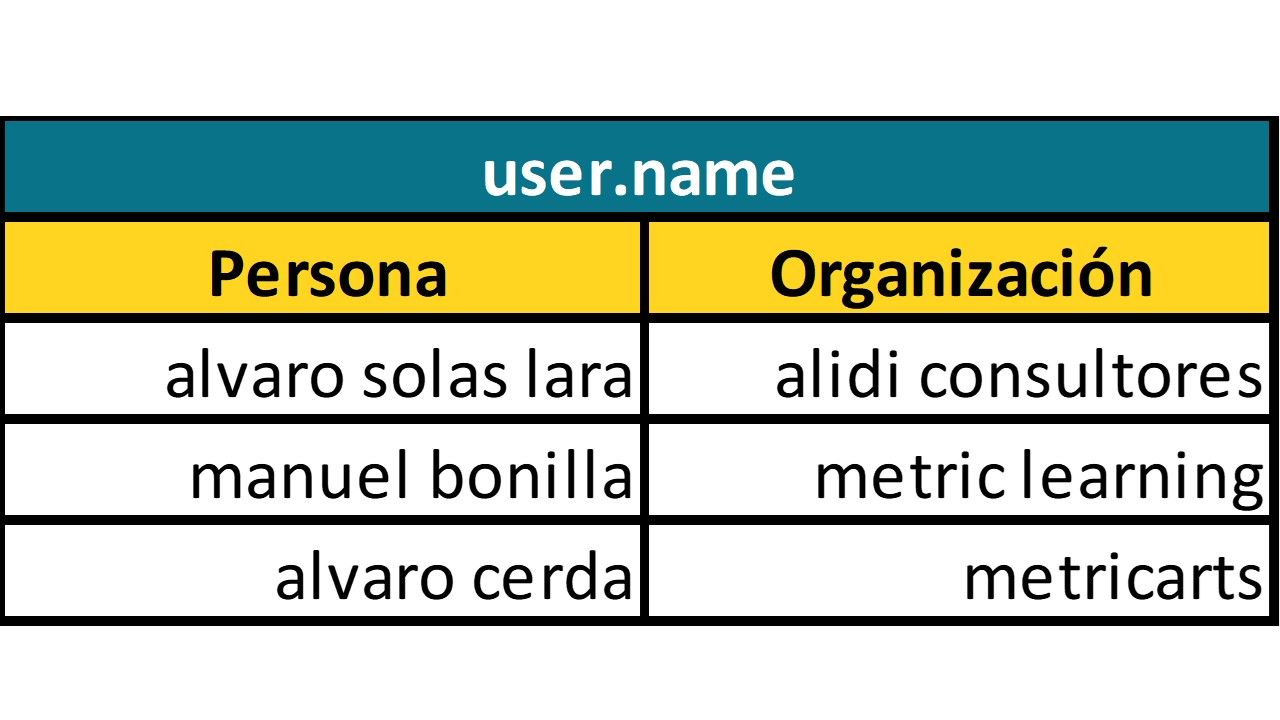
\includegraphics[width=0.4\textwidth]{Silvia_user_name_persona_organizacion}
\figcaption{Ejemplos de valores en el \lq\lq user.name\rq\rq.}
\label{fig:Silvia_user_name_persona_organizacion} }

Para aplicar el criterio {\bf E1} hemos manejado un archivo con nombres y apellidos 
de personas en español e inglés, obtenido de estas fuentes:
\begin{itemize}
\item\url{ https://www.census.gov/genealogy/www/%20data/1990surnames/names_files.html }
\item\url{
http://www.ine.es/dyngs/INEbase/es/operacion.htm?c=Estadistica_C&cid=1254736177009&menu=resultados&idp=1254734710990 }
\item\url{http://www.buscanombres.com/nombres-gallegos.htm }
\item\url{https://script.byu.edu/Pages/Spanish/es/surnames.aspx }
\end{itemize}
Para el caso de los nombres españoles se han incluido también los específicos para regiones como Cataluña, Comunidad Valenciana y Galicia. A pesar de la amplia lista de nombres y apellidos,
en muchos casos solo se identificaba el nombre, en otros solo los apellidos... Con lo que en lugar de validar a las personas con la coincidencia completa de su nombre de usuario, se determinó 
aceptar que es un nombre válido si se da una coincidencia del $33$\%. En aquellos casos en los que una 
persona incluye solo nombre y un apellido, sería suficiente con dejar el corte en el $50$\%,
pero cuando se publican nombre y dos apellidos,  es frecuente que solo detectemos el nombre y no los apellidos. De ahí que se tomara la decisión de fijar el umbral en el $33$\%.

\item Al inspeccionar el campo \lq\lq user.description\rq\rq encontramos ejemplos como
los siguientes:

\myfigure{
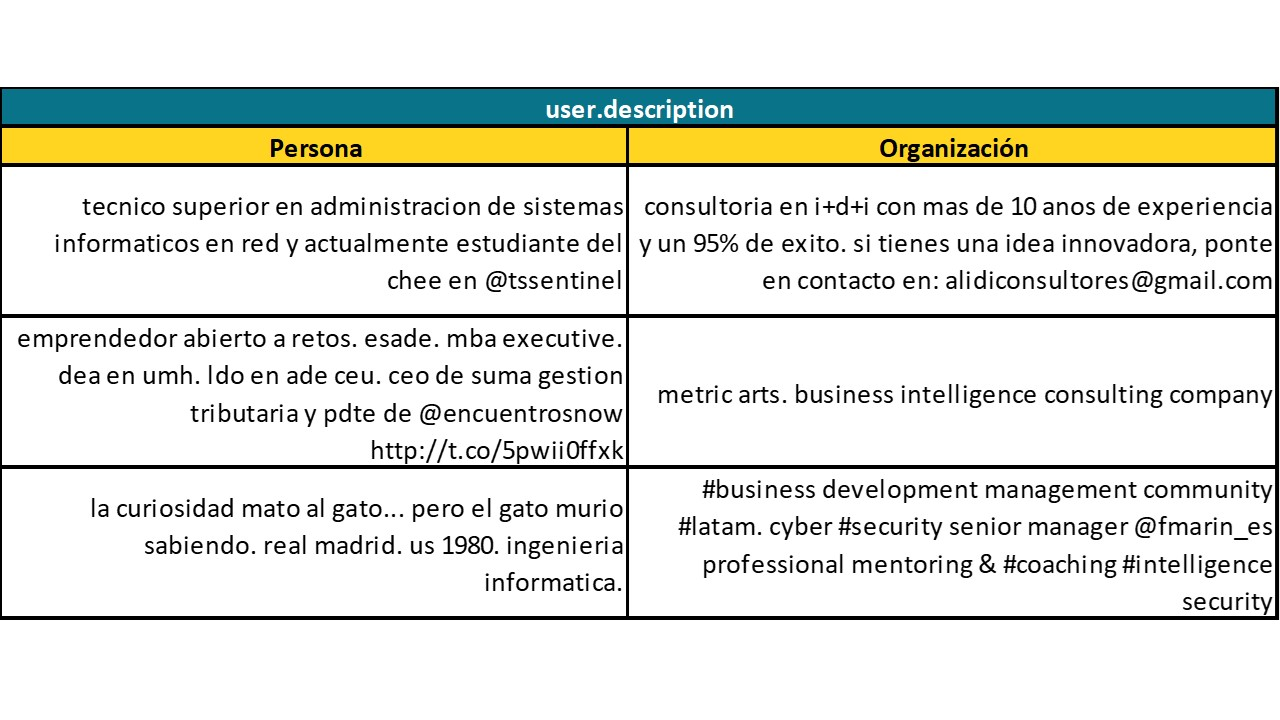
\includegraphics[width=0.8\textwidth]{Silvia_user_description_persona_organizacion}
\figcaption{Ejemplos de valores en el \lq\lq user.description\rq\rq.}
\label{fig:Silvia_user_description_persona_organizacion} }

Esta inspección, así como la realizada anteriormente a través de las nubes de palabras
de las figuras \ref{fig:bios_worldcloud2} y \ref{fig:bios_worldcloud},
nos sugieren que si aparecen palabras como \lq\lq emprendedor\rq\rq, \lq\lq consultor\rq\rq, 
\lq\lq profesional\rq\rq o \lq\lq persona\rq\rq, el  usuario es una persona. 
Se evitó poner las pa\-la\-bras \lq\lq I am\rq\rq o \lq\lq soy\rq\rq porque en el caso de 
algunos bots, en este campo aparecen textos si\-mi\-la\-res a \lq\lq I am a bot\rq\rq. 
Por otro lado, la aparición de palabras como \lq\lq negocio\rq\rq, \lq\lq empresa\rq\rq, 
\lq\lq compañía\rq\rq,\lq\lq somos\rq\rq, \lq\lq we\rq\rq\dots en el campo descripción o
en el campo nombre, indicarían que el usuario es una empresa u organización.
Se evitaron palabras como \lq\lq business\rq\rq por riesgo a que algunos pudieran 
publicar comentarios del área de {\em business intelligence}.
Tanto en el caso de las palabras que determinan personas, como de las que determinan
empresas, tanto en inglés como en español, se crearon sendos ficheros para su almacenamiento. 

\item Una primera inspección del campo \lq\lq url\rq\rq nos muestra estos ejemplos:

\myfigure{
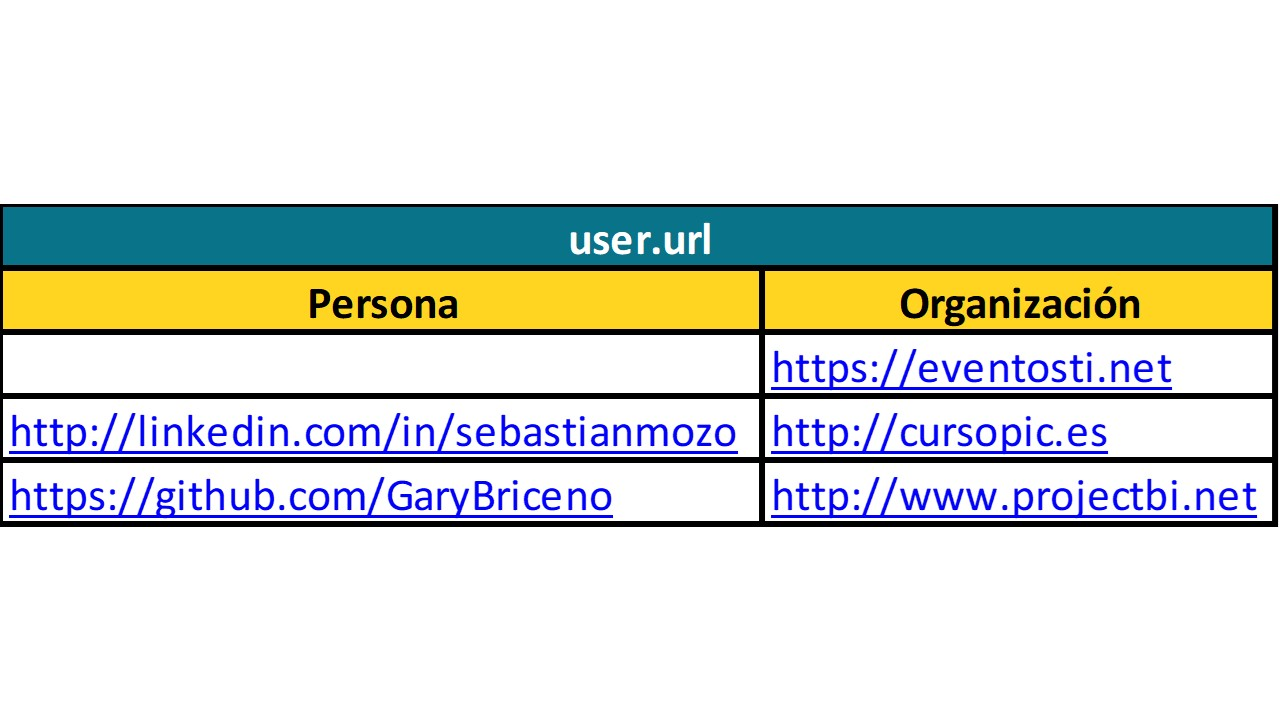
\includegraphics[width=0.8\textwidth]{Silvia_user_url_persona_organizacion}
\figcaption{Ejemplos de valores en el campo \lq\lq url\rq\rq.}
\label{fig:Silvia_user_url_persona_organizacion} }

En esta inspección descubrimos también que hay más empresas de las que cabría esperar, 
y fundamentalmente bots, cuyo campo url estaba vacío. No
nos parece entonces una buena característica para la clasificación. Sin embargo, sí que se atendió al hecho 
de que a veces en el campo url el usuario incluye en este campo su perfil de LinkedIn (con lo que el
texto \lq\lq linked\rq\rq aparece) o su blog personal (en cuyo caso podemos identificar el texto 
\lq\lq blog\rq\rq). Es cierto que en el caso de \lq\lq blog\rq\rq se puede incurrir en ciertos errores,
dado que también hay bots en cuyo campo url se incluye un blog y es uno de los puntos a mejorar. 

\item La idea apuntada sobre el origen de los tuits en la subsección  de la
página \pageref{subsubsect:origen_tuits}, que si el tuit era publicado desde un dispositivo de mano 
probablemente se trataría de una persona,  finalmente resultó que, de nuevo, no era la realidad y esa
diferenciación no era tan clara: más organizaciones de las que cabría esperar utilizaban dispositivos
de mano para publicar. Por tanto, el usar este campo como criterio único para la clasificación 
inmediata de personas tal y como proponen en \cite{user_class}, no nos daba buenos resultados. 
Ellos fundamentalmente lo utilizan para el caso en el que los usuarios no puedan ser clasificados
por alguno de los otros criterios debido a que no comparten información sobre su \lq\lq user.name\rq\rq 
o su \lq\lq user.description\rq\rq. Sin embargo, en nuestro caso, tan solo el $0.09$\% de los 
usuarios (sin repetición) no tienen nada en su campo descripción y un $0.2$\% en su campo nombre y tan solo 1 que no tiene ni en su campo descripción ni en su campo nombre. Por todo ello, rechazamos el criterio directo sobre el  origen.
\end{enumerate}

Con las observaciones anteriores se conseguía una buena clasificación de empresas y de personas. 
Los fallos en la clasificación de usuarios reales provenían sobre todo de tuits con nombres 
de usuario extraños o descripciones ambiguas, y fundamentalmente de etiquetar a bots como usuarios,  
pero no a causa de una mala clasificación entre personas y organizaciones.


Con respecto a las técnicas que queremos explorar para identificar aquellos usuarios
que sean bots, nos vamos a fijar en las siguientes características apuntadas en \cite{user_class6}:
\begin{itemize}
\item Frecuencia de tuiteo: dado que los bots suelen tuitear mucho, clasificaremos como
bots aquellos usuarios cuya frecuencia de publicación sea superior a un cierto umbral. No hay un 
nivel claro en el que situar dicho umbral. Este sería un punto a estudiar más profundamente y mejorar en un futuro. Nosotros hemos tomado el límite de $350$ tuits por día  desde la creación de la cuenta (lo que 
supone un tuit cada dos minutos con doce horas de actividad). 

\item Origen de los tuits: de acuerdo a los datos mostrados en la figura \ref{fig:sources}, se observa
que los principales orígenes de los tuits en nuestra muestra son \lq\lq Twitter Web Client\rq\rq, 
\lq\lq Twitter for Android\rq\rq y  \lq\lq Twitter for Iphone\rq\rq (Twitter para dispositivos de 
mano en los dos últimos casos). Vamos a considerar como bots aquellos tuits producidos desde: 

\begin{tabular}{cccc} 
\lq\lq IFTTT\rq\rq,  &\lq\lq Roundteam\rq\rq,  &\lq\lq Botize\rq\rq, &\lq\lq  Statistics for IT\rq\rq,\\
 \lq\lq  Koica Retweeter\rq\rq, &\lq\lq Tweet Old Post\rq\rq, &\lq\lq Powerapps and Flow\rq\rq, &\lq\lq Voicestorm\rq\rq. 
\end{tabular}

Todos ellos están descritos en la página \pageref{page:sources_descriptions}.

\item Por último, hemos visto que lo más directo es eliminar a aquellos bots que se identifican 
como tales a través de alguno de los campos \lq\lq user.name\rq\rq, \lq\lq user.description\rq\rq o \lq\lq source\rq\rq. De estos tres campos finalmente descartamos el de \lq\lq user.description\rq\rq ya que en el ámbito de la tecnología (al cual pertenecen nuestro perfiles) existen menciones a la palabra "robotica". 
\end{itemize}
A continuación mostramos algunos ejemplos de datos en nuestra muestra, en los que se aprecian
las observaciones anteriores:

\myfigure{
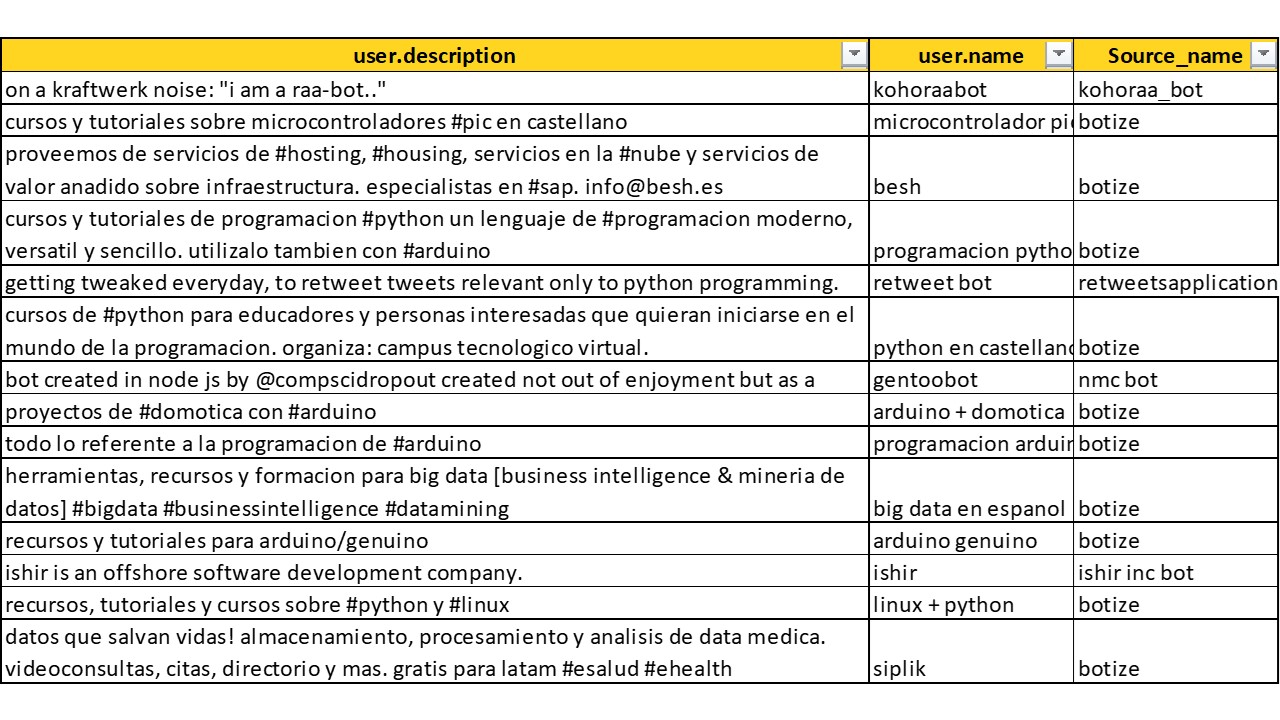
\includegraphics[width=0.8\textwidth]{Silvia_bots}
\figcaption{Ejemplos de valores.}
\label{fig:Silvia_bots} }

\subsection{Modelo final}

En vista de todas estas observaciones, el algoritmo que hemos usado toma la siguiente forma:
un tuit se considera de una persona cuando 
\begin{itemize}
\item en su campo nombre de usuario existe un $33$\% o más 
de coincidencia con la lista de nombres y apellidos, 
\item {\bf y} si en su descripción de usuario aparece algún término que
identificamos como de persona {\bf o} no aparecen términos 
relacionados con empresa ni en la descripción del usuario ni en el nombre de usuario.
\item {\bf y} la frecuencia de publicación de tuits es inferior a $350$
\item {\bf y} el origen de tuit no es uno de los que identificamos como automáticos
\item {\bf y} la palabra \lq\lq bot\rq\rq no aparece ni en el nombre del usuario ni
en el nombre del origen del tuit,
\item {\bf o bien}  cuando su url es una url de LinkedIn o de un blog.
\end{itemize}

El código para llevar a cabo esta limpieza estaría preparado para escalar
el modelo a otros casos de uso. Por ejemplo:
\begin{itemize}
\item la lista de nombres y apellidos puede extenderse fácilmente para incluir nombres
en otros idiomas, si resulta que el texto de las descripciones o de los tuits recolectados
se clasifica en otros lenguajes además del inglés y el español, o para extender el alcance de
detección del modelo.
\item De igual forma, en la lista de términos que sí pueden aparecer en descripción, donde ahora
incluimos fundamentalmente vocablos relacionados con perfiles técnicos (consultor, matemático, ingeniero, etc.)
para clasificar los usuarios como personas, se puede modificar fácilmente para incluir aquellos que estén 
relacionados con el perfil requerido en la oferta laboral y mejorar la clasificación.
\item Respecto a la lista de términos que no deben aparecer en el campo descripción (porque identifican empresas 
o bots) se podría utilizar sin ningún cambio. En el caso en el que los tuits sean en otros idiomas diferentes 
al inglés o al español se podría incluir fácilmente la versión en los idiomas necesarios de las palabras 
consideradas.
\item La lista de aplicaciones identificadas como productoras de tuits automatizados también
está consignada en un fichero fácilmente modificable.
\end{itemize}

\subsection{Evaluación del modelo}
Para evaluar la precisión del modelo hemos etiquetado manualmente $1364$ de los registros que 
teníamos que clasificar(en el fichero 
{\bf Detect\_Pers/Filtro\_pers\_30\_01.xlsx} de nuestro repositorio de GitHub se pueden encontrar
dichos datos), 
y hemos calculado la matriz de confusión (figura \ref{fig:confussion_matrix_definition} 
de la sección \ref{sect:ajuste_modelo_contenido_tuit}) de los resultados de aplicar el
modelo de clasificación anterior a esos datos etiquetados. Es la siguiente:

\begin{center}
\begin{tabular}{r|cc}
\multicolumn{3}{c}{\bf Matriz de confusión} \\
\hline
\hline
     &$1$&$0$\\
\hline
$1$&$687$&$110$\\
\hline
$0$&$26$&$541$\\
\hline
\end{tabular}
\end{center}

A partir de esta matriz de confusión, y siendo el $N$ el total de las observaciones,
calculamos las siguientes métricas para el modelo:
\begin{itemize}
\item Exactitud (\lq\lq accuracy\rq\rq): $\displaystyle Ac =\frac{TP+TN}{N} = 90$\%	
\item Tasa de error (\lq\lq misclassification \rq\rq): $\displaystyle TE =\frac{FP+FN}N = 10$\%
\item Sensibilidad (recall), tasa de verdaderos positivos:												
$\displaystyle Rc =\frac{TP}{TP+FN}= 86,2$\%
\item Especificidad, tasa de verdaderos negativos:														
$\displaystyle Es =\frac{TN}{TN+FP}= 95,4$\%			
\item Precisión:													
$\displaystyle Pr =\frac{TP}{TP+FP}= 96,4$\%	
\item Valor de predicción del tipo negativo:
$\displaystyle VPN =\frac{TN}{TN+FN}= 83,1$\%										
\end{itemize}														
														
Observamos que la proporción mayor de mal clasificados está en personas que no han sido 
clasificadas como tal. Un porcentaje se debe a personas con falta de información  en su bio 
o cuya descripción del perfil profesional no es acorde con los perfiles buscados. 
Con estos resultados, aceptamos el modelo propuesto.

% Realmente muchos de ellos se solucionan al seleccionar usuarios a través del tema tratado.

% Por otro lado, \lq\lq Voicestorm\rq\rq se incluyó como filtro para clasificar como \lq\lq no persona\rq\rq
% cuando debería ser al contrario. El impacto es pequeño ya que solo hay $26$ usuarios que utilizan este 
% origen,  pero hay que tenerlo en cuenta para futuras clasificaciones.

\subsection{Eliminación de duplicados}
\label{subsect:duplicados2}
Una vez obtenida la clasificación en persona o no persona de los usuarios llevada a cabo como
hemos descrito, solamente nos queda producir el listado definitivo de candidatos seleccionados 
(ya no va a haber ninguna clasificación posterior). Esto implica, en primer lugar, que eliminaremos
de la lista aquellos usuarios que no han sido clasificados como persona. A continuación, nos interesa
extraer las personas únicas que hemos detectado: del listado extraído del paso anterior, 
sección \ref{subsect:duplicados1}, podría ocurrir que un usuario  fuera clasificado como persona con un
conjunto de url, nombre de usuario y descripción, pero no lo fuera con otro. En esta fase, por tanto, nos limitaremos a eliminar del listado de los clasificados como personas aquellos usuarios con un id repetido.

\subsection{Resultados de la selección}
Aplicando esta metodología a la lista de usuarios únicos obtenidos tras la aplicación
de los algoritmos descritos en la sección \ref{sect:tuits_relevantes}, 
hemos obtenido los siguientes datos: de $231$ usuarios únicos analizados, 
hemos encontrado $155$ que clasificamos como 
personas, lo que representa un $67.1$\%  del total, y de éstos
no había ninguno cuyo \lq\lq user\_id\rq\rq estuviera duplicado. Los resultados relativos están consignados en la siguiente gráfica:

\myfigure{
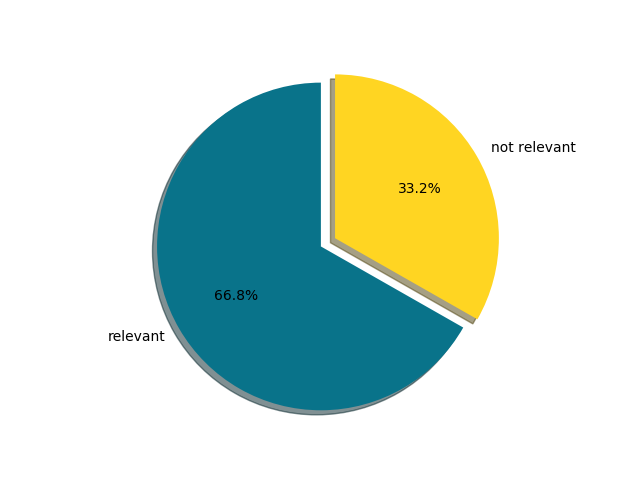
\includegraphics[width=0.6\textwidth]{C:/DATOS/MBIT/Proyecto/MBITProject_Data4all/Python/images/relevant_users_proportion.png}
\figcaption{Porcentaje de usuarios clasificados como personas.}
\label{fig:relevant_users_proportion} }


Los siguientes usuarios fueron clasificados como no personas:


\myfigure{
\begin{tabular}{ccc}

\includegraphics[width=0.2\textwidth]{not_person1}
&
\includegraphics[width=0.2\textwidth]{not_person2}
&
\includegraphics[width=0.2\textwidth]{not_person7}\\

\includegraphics[width=0.2\textwidth]{not_person4}
&
\includegraphics[width=0.2\textwidth]{not_person8}
&
\includegraphics[width=0.2\textwidth]{not_person6}\\

\includegraphics[width=0.2\textwidth]{not_person3}
&
\includegraphics[width=0.2\textwidth]{not_person5}
&
\includegraphics[width=0.2\textwidth]{not_person9}
\end{tabular}
\figcaption{Usuarios no clasificados como persona.}
\label{fig:users_not_persons} 
}


Y los siguientes son algunos de los que se clasificaron como persona:


\myfigure{
\begin{tabular}{cccc}

\includegraphics[width=0.2\textwidth]{person1}
&
\includegraphics[width=0.2\textwidth]{person4}
&
\includegraphics[width=0.2\textwidth]{person3}
&
\includegraphics[width=0.2\textwidth]{person2}
\end{tabular}
\figcaption{Usuarios clasificados como persona.}
\label{fig:users_persons} 
}

En el siguiente capítulo explicamos cómo ordenamos estos $155$ usuarios.
